\documentclass{article}

\usepackage{amsmath, graphicx}

\graphicspath{ {./images/} }

\title{Ch. 27 CW Solutions}
\author{Principles of Macroeconomics}
\date{\today}

\begin{document}

\maketitle

\begin{enumerate}

\item

	\begin{enumerate}
	
	\item The stock price will go up because perception of the firm's future profitability will improve.
	
	\item The stock price will decrease because lower profit than expected this year will dampen expectations of profit in the future.
	
	\item The stock price will decrease because if the industry as a whole is doing poorly, perception of the firm's future profitability will worsen. 
	
	\item The stock price won't change because perception of the firm's future profitability won't change.
	
	\end{enumerate}
	
\item
	\begin{gather*}
	S_{Priv} = Y - T - C = \$20,000 - \$1,700 - 14,000 = \$4,300 \\
	S_{Pub} = T - G = \$1,700 - \$2,500 = -\$800 \\
	S_{Nat} = S_{Priv} + S_{Pub} = \$4,300 - \$800 = \$3,500 \\
	I = S_{Nat} = \$3,500
	\end{gather*}
	
\item

	\begin{enumerate}
	
	\item It should. If the firm did its next best option and saved the money, it would make $0.1(\$4,500) = \$450$ per year. That's less than it would make if it bought the machine. 
	
	\item No, it makes the machine a bad investment. The firm would make $0.12(\$4,500) = \$540$ per year if it saved the money. That's more than it would make if it bought the machine.
	
	\item A higher interest rate discourages investment and encourages saving. 
	
	\item The firm should be willing to pay up to \$5,000. That's the price at which the revenue it makes from buying the machine equals the interest it would make from saving the money, $0.1(\$5,000) = 500$.
	
	\end{enumerate}
	
\item

	\begin{enumerate}
	
	\item When the government cuts spending, it increases national saving, and that shifts the supply of loanable funds right. That decreases the interest rate and increases the amount of saving and investment in the economy. 
		\begin{center}
		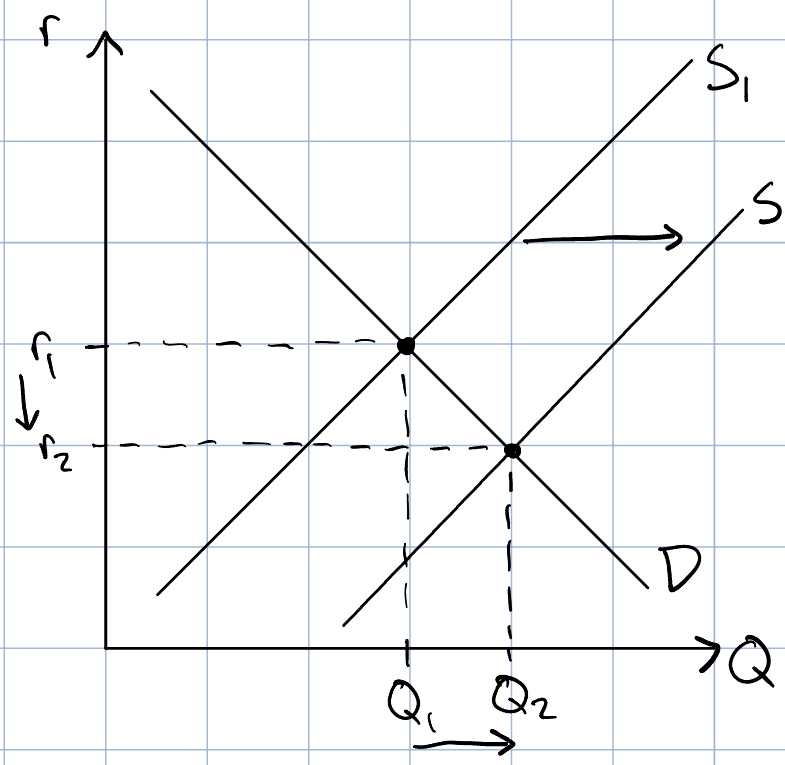
\includegraphics[width = 0.5\textwidth]{4a}
		\end{center}
	
	\item Higher taxes decrease corporate profits, and that decreases firms' incentive to invest. The demand for loanable funds shifts left, the interest rate decreases, and the amount of saving and investment in the economy decreases.
		\begin{center}
		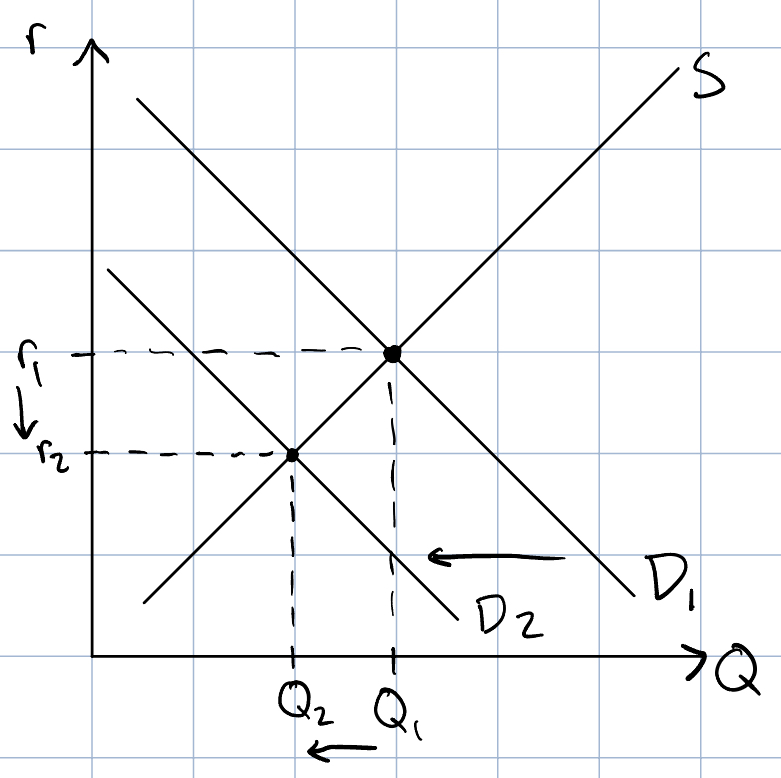
\includegraphics[width = 0.5\textwidth]{4b}
		\end{center}
	
	\item A decrease in saving shifts the supply of loanable funds to the left. That increases the interest rate and decreases the amount of saving and investment in the economy. 
		\begin{center}
		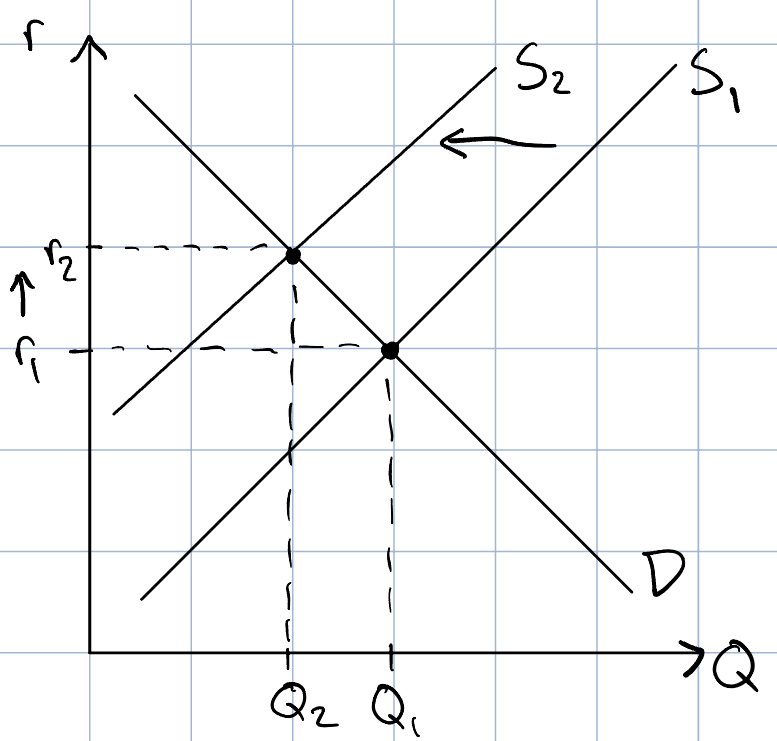
\includegraphics[width = 0.5\textwidth]{4c}
		\end{center}
	
	\item When capital becomes more productive, it increases firms' incentive to invest. The demand for loanable funds shifts right which increases the interest rate and increases the amount of saving and investment in the economy.
		\begin{center}
		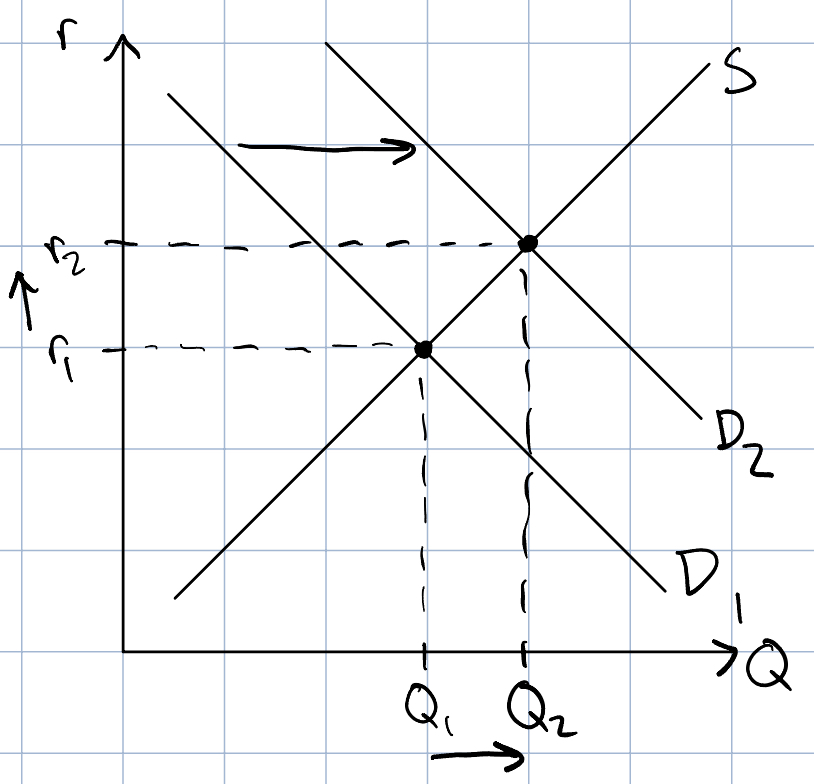
\includegraphics[width = 0.5\textwidth]{4d}
		\end{center}
	
	\item If capital becomes more costly to operate, it disincentivizes firms from investing, so the demand for loanable funds shifts left. That decreases the interest rate and the amount of saving and investment in the economy.
		\begin{center}
		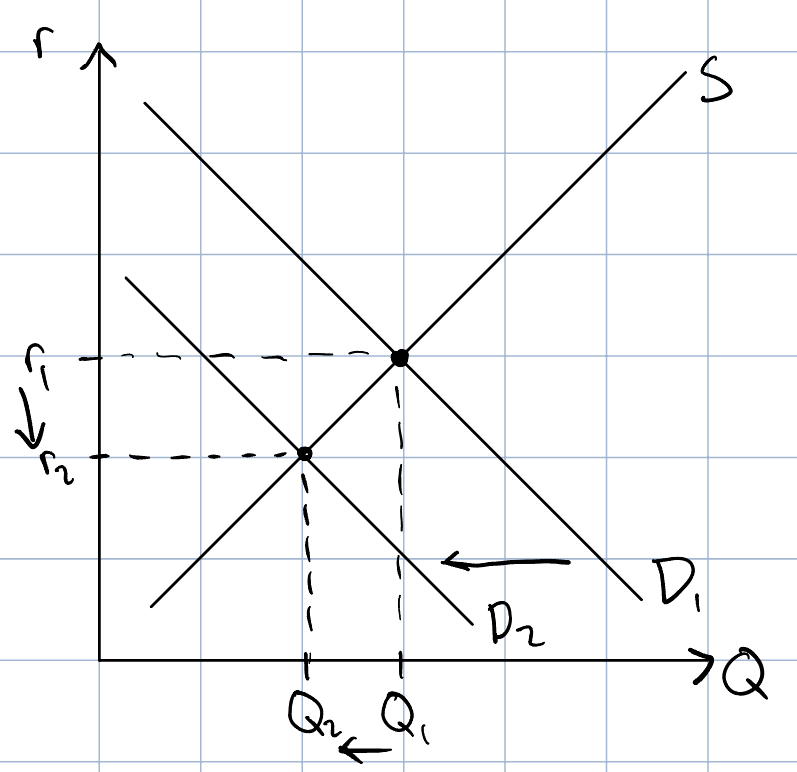
\includegraphics[width = 0.5\textwidth]{4e}
		\end{center}
	
	\item If the government cuts taxes on corporate profits, firms have more of an incentive to invest, so the demand for loanable funds shifts right. If the government cuts taxes but not spending, public saving will decrease which shifts the supply of loanable funds left. As a result, the interest rate increases, but the change in saving and investment is ambiguous.
		\begin{center}
		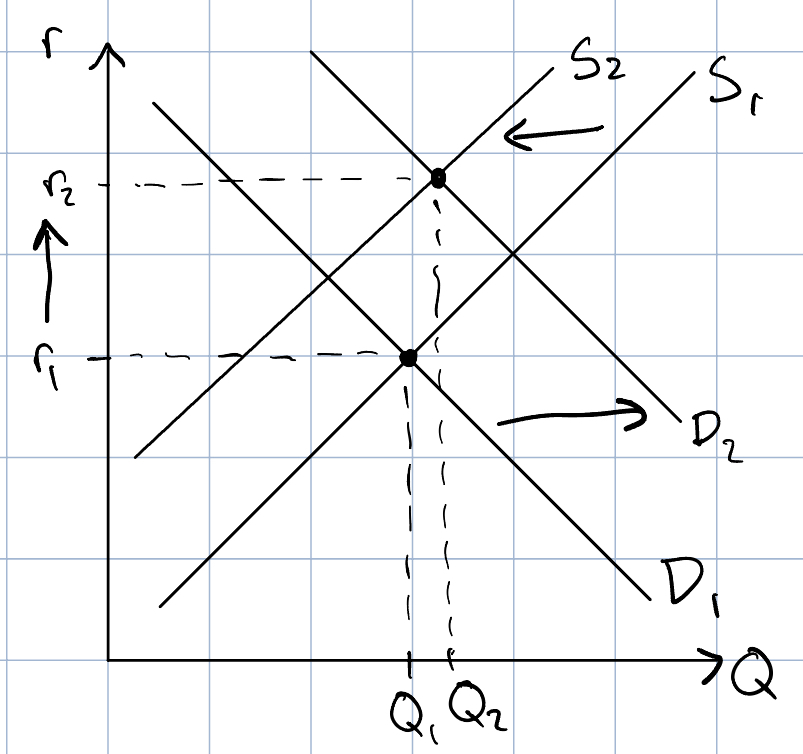
\includegraphics[width = 0.5\textwidth]{4f}
		\end{center}
	
	\end{enumerate}

\end{enumerate}

\end{document}